% DAC Paper
\documentclass{sig-alternate}
\usepackage{subfigure}

\pagestyle{empty}

%
\begin{document}

% Do not want to print date
\date{}

\title{A System For Coarse Grained Memory Protection In Tiny Embedded Processors}

\numberofauthors{1}
\author{
\alignauthor Ram Kumar, Akhilesh Singhania, Andrew Castner, Eddie Kohler, Mani Srivastava \\
	\affaddr{University of California at Los Angeles}\\
	\affaddr{420 Westwood Plaza, Los Angeles, CA, USA}\\
	\email{\{ram,akhi,mbs\}@ee.ucla.edu, \{castner,kohler\}@cs.ucla.edu}
}

\maketitle
\thispagestyle{empty}


\begin{abstract}
%==============================================================
% ABSTRACT
%==============================================================
\noindent
Many embedded systems contain resource constrained microcontrollers where applications, operating system components and device drivers reside within a single address space with no form of memory protection.
%
Programming errors in one application can easily corrupt the state of the operating system and other applications on the microcontroller.
%
In this paper we propose a system that provides memory protection in tiny embedded processors\footnote{8, 16 and 32-bit microcontrollers with limited resources}.
%
Our system consists of a software run-time working with minimal low-cost architectural extensions to the processor core that prevents corruption of state by buggy applications.
%
We restrict memory accesses and control flow of applications to \textit{protection domains} within the address space.
%
The software run-time consists of a \textit{Memory map}: a flexible and efficient data structure that records ownership and layout information of the entire address space.
%
Memory map checks are done for \texttt{store} instructions by hardware accelerators that significantly improve the performance of our system.
%
We preserve control flow integrity by maintaining a \textit{Safe stack} that stores return addresses in a protected memory region.
%
Cross domain function calls are redirected through a software based jump table.
%Domain switches within a single address space is done with the help of a cross domain linker tool that generates a software jump table.
%
Enhancements to the microcontroller \texttt{call} and \texttt{return} instructions use the jump table to track the current active domain.
%
We have implemented our scheme on a VHDL model of ATMEGA103 microcontroller.
%
Our evaluations show that embedded applications can enjoy the benefits of memory protection with minimal impact on performance and a modest increase in the area of the microcontroller.

\end{abstract}
%

\vspace{1mm}
\noindent
{\bf Categories and Subject Descriptors:} C.3 {[Special - \\Purpose and Application-Based Systems]}: {Real-time and embedded systems}

\vspace{1mm}
\noindent
{\bf General Terms:} Performance, Design, Reliability

\vspace{1mm}
\noindent
{\bf Keywords:} Memory Protection, HW SW Codesign

%%%%%%%%%%%%%%%%%%%%
% INTRODUCTION
%%%%%%%%%%%%%%%%%%%%
\section{Introduction}
\label{sec:introduction}
%
This paper explores the challenges in providing fault isolation
through memory protection on resource constrained embedded systems
such as sensor nodes.
%
%Sensor networks have promise for many industrial, commercial, and
%medical applications.
%
%For example, CodeBlue~\cite{welsh04codeblue} is a prototype medical
%sensor network platform for expediting triage during disaster
%response.
%
%A network of 4000 sensors deployed by Intel in a
%semiconductor fabrication plant performs predictive maintenance of
%machinery in service~\cite{intel05fabapp}.
%
%The Zigbee consortium~\cite{zigbee} seeks to equip lighting and
%HVAC controllers with wireless radios, enabling intelligent building
%automation and security services.
%
%These 
Current and upcoming sensor network deployments require high
availability infrastructure with the ability to support multiple users.
%
%
Unexpected system failures could cause problems ranging from financial
impacts to loss of life.
%
Current software technology is grossly inadequate to run such long
term deployments.
%
Bugs in any part of the software can easily bring down an entire network.
%
In particular, memory corruption due to buggy applications can crash or
freeze sensor nodes or corrupt sensed data.
%
We argue that memory protection is a vital enabling technology for
creating reliable and long-lasting sensor network software systems.
%

Sensor software is quite complex, supporting 
%
many sensor types, multiple distributed
middleware services, dynamic code updates, and concurrent applications.
%
Programmers must deal with severe resource constraints and concurrency issues
%
on hardware with very limited debugging support.
%
Therefore, programming errors are quite common and can impact the network.


Mote-class sensor nodes~\cite{jasonhillthesis} have a very simple architecture.
%
All primary memory is accessible to all programs running
on a node via a single address space.
%
Common mote-class architectures do not have features such as memory
management units (MMUs) and privileged-mode execution used in
desktop/server class systems to isolate program data and code.
%
Embedded microcontroller designers face extreme pressure to minimize chip cost and area.
%
Sometimes even 32-bit ARM processor cores omit an MMU to minimize system cost and power~\cite{arm7tdmi}.
%
We expect MMU designs will continue to be absent from low-cost low-power
microcontrollers.
%
Therefore, there is a need for new advancements in software and architecture
technology to make robust sensor node applications.
%
%==================================================================
%\subsection{Memory Protection in Embedded Sensor Systems}
%
%Software-based approaches for memory protection have emerged to
%compensate for the architectural limitations of embedded
%microcontrollers.
%
%Domain specific interpreters such as Mat\'e~\cite{asvm05nsdi} provide
%a safe environment to execute high-level application scripts.
%
%Type-safe languages such as Virgil~\cite{titzer06virgil} provide
%fine-grained protection of individual memory objects.
%
%However, these approaches have their limitations.
%
%For example, Mat\'e instructions are implemented in non type-safe
%language and could be buggy.
%
%Type-safe languages require unsafe extensions to interface to the
%low-level hardware, though these extensions could be used sparingly.
%
%An ideal system for memory protection might combine two or
%more software-based approaches.
%


In this paper, we present \emph{Harbor}, a system for providing
%software-based 
coarse-grained memory protection in resource-%
constrained embedded sensor nodes.
%
%Harbor can be used as a building block with other approaches to create
%more effective protection mechanisms.
%
%For instance, Harbor can be used to implement memory safe Mat\'e
%instructions.
%
Harbor partitions a sensor node's memory into
multiple \textit{domains}.
%
Memory belonging to one domain is protected from corruption by code running
in other domains.
%
We achieve memory protection by enforcing restrictions on memory accesses.
%
In this paper, we have designed two systems that introduce these restrictions.
%
The first system re-writes machine instructions of a compiled binary.
%
This software only technique, first proposed by Wahbe et
al.~\cite{wahbe93sfi}, is known as software-based fault isolation,
SFI, or ``sandboxing''.
%
The second system modifies the processor architecture to enforce memory
access restrictions and is applicable to system-on-chip embedded
systems using processor cores.
%

%==================================================================
\subsection{Contributions of the Paper}
%
We improve the reliability of embedded sensor software by isolating
the domains from one another.
%
This paper investigates the challenges in implementing fault isolation
on resource-constrained embedded sensor nodes.
%
Scarce memory resources require Harbor to have a very small memory
footprint.
%
Limited computational capabilities also encouraged us to limit Harbor's
CPU overhead.
%
The contribution of our work has been to design techniques that make
sandboxing feasible on embedded sensor nodes despite these
constraints.
%
In particular, these techniques are:
%
\begin{itemize}
%
\item{A \emph{Memory map} data structure that efficiently maintains
fine-grained ownership and layout information for the entire address
space.
%
Motes' limited address space precludes static address space
partitioning: there is not enough memory available to assign each
domain a single contiguous range of addresses.
%
The memory map can be tuned to match available resources and protection
requirements.
%
}
%
\item{A \textit{Safe stack} in protected memory preserves control flow
integrity~\cite{xfi06osdi} within a domain by storing function return addresses.
%
The conventional run-time stack, which stores local data, function
parameters, and so forth and is shared by all the domains, is
protected from corruption via \emph{stack bounds}.
%
The alternative of maintaining a separate stack per
domain is not desirable due to address space limitations.
%
}
%
\item{\textit{Cross domain calls} implement low-overhead
context switches between domains.
%
The overhead of copying call arguments is eliminated as the domains
share a common run-time stack.
%
Cross domain calls and returns track the system's currently active domain.
%
}
%
\item{\textit{Run-time checks} ensure that control flow in and out
of a domain occur as expected even on computed transfers, and
similarly that memory is accessed only as expected.
%
}
%
\end{itemize}

%Figure~\ref{fig:sys_comp} presents the components of the Harbor memory
%protection system and the interactions between them.
%
These techniques are easily incorporated into existing systems.
%
We have designed and evaluated two systems that use the Harbor fault isolation
techniques.
%
Our experiments show that memory protection through fault isolation is
feasible on resource constrained sensor nodes.

% \begin{figure}[htbp]
%     \centering
%     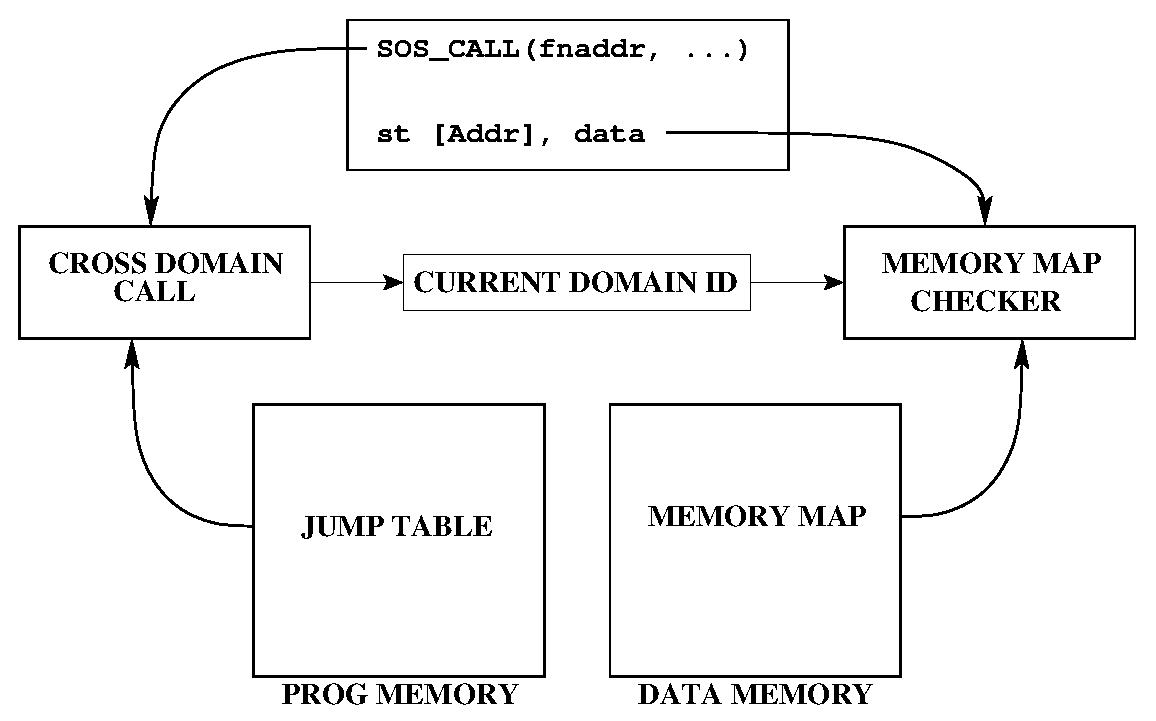
\includegraphics[height = 2.5in, keepaspectratio=true]{figures/syscomp.eps} 
%     \caption{Components of Harbor Memory Protection}
%     \label{fig:sys_comp}
%  \end{figure}

%-------------------------------------------------------
\subsection{Applications of Harbor Memory Protection}
%
\subsubsection{Memory Protection in SOS Operating System}
%
SOS~\cite{ram05sos} is an operating system for sensor nodes in which a
statically compiled kernel is installed on the node, and application
level functionality is implemented by a set of dynamically loadable
binary modules.
%
We use Harbor memory protection to isolate binary modules running
on SOS.
%
Run-time checks are introduced in a SOS module by a \emph{binary rewriter} and
verified independently by a \emph{verifier} running on every sensor
node.
%
To minimize the module code size, the run-time checks are not inlined.
%
Modules invoke the run-time checks by calling or jumping into the
appropriate routines located in the trusted domain (the SOS kernel).
%
%% Thus, it is not possible to circumvent checks as 
All potentially unsafe operations such as stores to memory are replaced
by calls to corresponding checks.
%
%Calls to the checks are introduced by a \emph{binary rewriter} and verified
%independently by a \emph{verifier} running on every sensor node.
%
Harbor's correctness depends only upon the correctness of the
verifier and the Harbor runtime, and not on the rewriter.
%
%The design of the verifier affects the system's performance
%(Section~\ref{sec:writeverify}).
%
%So far, we have only 
We have designed a simple verifier that requires constant state
information for a binary.
%
%Exploring the design space of verifiers and evaluating their impact on
%performance is a challenge that remains to be addressed.
%----------------------------------------------------------------------------
\subsubsection{Micro Memory Protection Unit}
%
We design a Micro Memory Protection Unit (UMPU) by partitioning the
Harbor Memory Protection system into hardware and software components.
%
UMPU was implemented on the AVR~\cite{avrdatasheet} microcontroller and
its performance was evaluated by executing complex software systems
such as SOS.
%
The careful hardware software co-design of UMPU results in significant
performance improvement over a software-only implementation with minimal
increase to the area and cost of AVR.
%
AVR enhanced with UMPU extensions is instruction set compatible with
regular AVR microcontrollers.
%
This design feature has practical value, as the existing
toolchains for the AVR architecture can be used with UMPU.
%
%
%An additional benefit of UMPU is that it eliminates the binary
%rewriting required by the software-only implementation that can be
%error-prone.
%


During experimentation, Harbor detected memory corruption in a data
collection application module that had been in use for several months.
%
A common programming mistake in SOS is to forget to check the error code
returned by a cross-domain function call.
%
In the Surge data collection module~\cite{woo03surge}, under certain
conditions, the invalid result of a failed function call to the Tree
routing module was being used to determine an offset into a buffer.
%
Subsequently, the data was being written to an incorrect memory
location, which would cause some of the nodes in the network to crash.
%
Harbor was successfully able to prevent the corruption and signal the
invalid access.
%


The cross-domain function call described above fails under the rare
condition when the Surge module is loaded on a node before the Tree
routing module.
%
Such conditions can be easily missed during software testing.
%
However, during deployments, the errors caused due to such failures
can have a severe impact on the network.
%
A system that can guarantee memory protection is indispensable for
building robust embedded software.
%

Harbor protection mechanism can be applied in general to a large class
of resource constrained embedded systems.
%
In this paper, we will focus primarily on the application of Harbor
protection to embedded sensor networks.
%
%----------------------------------------------------------------------------
%
%\subsection{Robust Embedded Software}
%
%============================================================
\subsection{Structure of Paper}
%
This paper is structured as follows.
%
Section~\ref{sec:related} gives an overview of related work,
examining previous work on software reliability in sensor networks,
software based fault isolation techniques and hardware based
approaches to memory protection in embedded and desktop systems.
%
%There is also a background on the SOS operating system. 
%and presents an overview of the Harbor memory
%protection primitives and their role in
%system that is designed to sandbox 
%sandboxing the dynamically loadable SOS modules.

Section~\ref{sec:memmap} explains the memory map data structure, which
contains fine grained ownership and layout information for every block
within the address space of the sensor node. 
%
Section~\ref{sec:cfmgr} discusses the Control Flow Manager, which
ensures the integrity of control flow within a protection domain
despite memory corruption localized to a domain.

Section~\ref{sec:writeverify} describes the design and implementation
of a binary rewriter tool that sandboxes SOS modules.
%
The sandboxed modules interact with the Harbor run-time components.
%
There is a detailed discussion on the design space of the verifiers
for a binary rewriter.

Section~\ref{sec:umpu} describes the components of UMPU.
%
There is an in-depth 
%detailed design 
description of all the functional units
within UMPU and their interaction with the software library.

We present detailed performance and resource consumption analysis of
Harbor and UMPU in Section~\ref{sec:eval}.
%
We conclude with a summary of our findings and directions for future
work in Section~\ref{sec:conclude}.

%==========================================================================
% DESIGN COMPONENTS
%==========================================================================
\section{Memory Map}
\label{sec:memmap}
%
%==========================================================================
% PROTECTION DOMAINS
%==========================================================================
%
\subsection{Protection Domains}
%
Our \textit{fault model} for memory protection is the corruption of state belonging to a module caused due to illegal write operations made by some another module.
%
We create and enforce \emph{Protection Domains} within data memory address space of the embedded processor.
%
Protection domain refers to a fragmented but logically distinct portion of overall data memory address space (Figure ~\ref{fig:prot_domains}).
%
Every module stores its state in its own protection domain.
%
No assumptions are made about layout of state within a domain.
%
Modules are restricted from writing to memory outside their domain through run-time checks.
%
There is one single trusted domain in the system that is allowed to access all memory.
%

Protection models based on domains do not address all possible memory corruption faults in the system.
%
Modules can still corrupt their own state as it resides completely within a protection domain. 
%
This form of corruption, though undesirable, is less serious than corruption across domains.
%
If we have an operating system we can load the kernel image in its separate domain.
%
A stable kernel can always ensure a clean re-start of user modules when corruption is detected.
%
\begin{figure}[htbp]
   \centering
   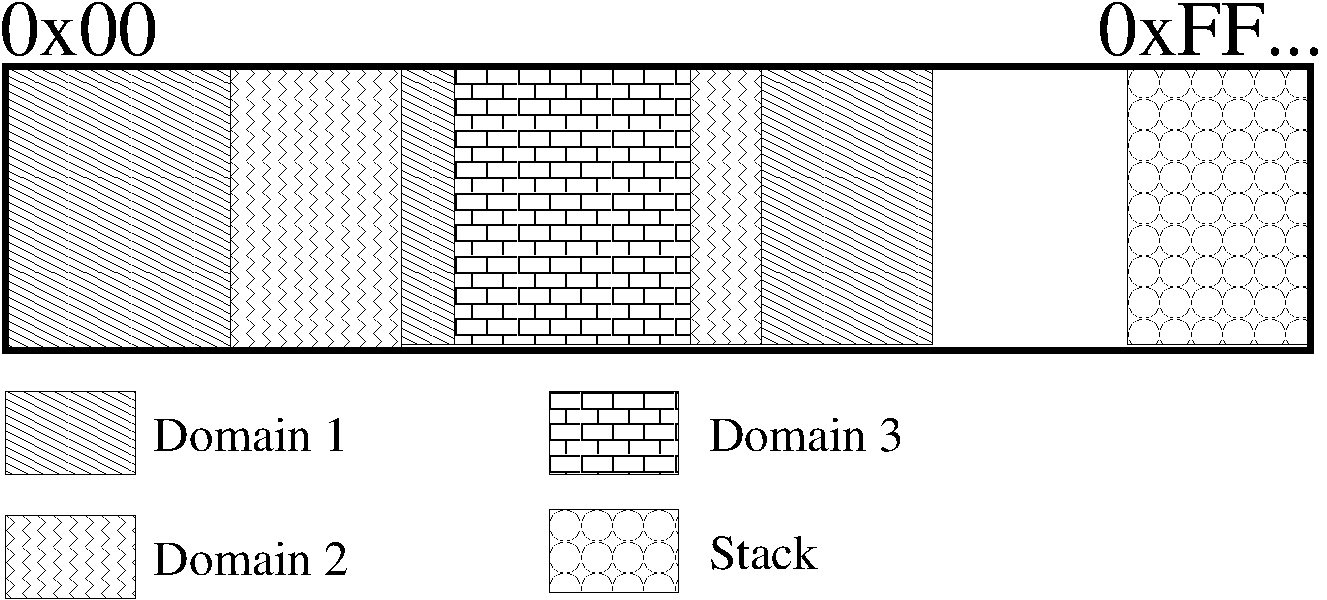
\includegraphics[height = 1in, keepaspectratio=true]{figures/domains.pdf} 
   \caption{Protection Domains}
   \label{fig:prot_domains}
\end{figure}
%
%========================================================================================================================================
% MEMORY MAP DATA STRUCTURE
%========================================================================================================================================
\subsection{Memory Map Data Structure}
%
%
Creating and enforcing protection domains is a challenging task on resource constrained embedded platforms.
%
Limited memory prohibits static contiguous partitioning of address space into multiple domains.
%
Instead we partition the address space of the microcontroller into blocks of equal sizes.
%
A \textit{Block} is a small contiguous region of memory.
%
Memory is allocated to domains as \textit{segments}, which are simply sets of contiguous blocks.
%
Allocation of segments to domains could be static (at compile time) or dynamic (through a memory heap).
%
A domain could be allocated multiple segments that are scattered randomly across entire address space.
%
\textit{The Memory Map contains access permissions for every block of address space.}
%
The Memory Map specifies two pieces of information.
% 
First, it contains ownership information (domain identity) for every block of memory.
%
Second, it encodes information about memory layout such as start of a logical segment of allocation to programs.
%
An example of actual encoded information and their meaning is specified in Table~\ref{tab:mmap_table}.
%
\begin{table}[htdp]
\centering
\small{
\begin{tabular}{|c|l|}
	\hline
	Code & Meaning\\
	\hline
	1111 & Free or Start of Trusted Segment\\
	1110 & Later portion of Trusted Segment\\
	xxx1 & Start of Domain (0 - 6) Segment \\
	xxx0 & Later portion of Domain (0 - 6) Segment\\
	\hline
\end{tabular}}
\caption{Encoded information in memory map table for multi-domain protection}
\label{tab:mmap_table}
\end{table}
%
%
%========================================================================================================================================
% MEMORY MAP CHECKER
%========================================================================================================================================
\subsection{Memory Map Checker}
%
A memory map checker is required to validate memory accesses made by software components.
%
It enforces the protection model that we described earlier; programs can write only into their domain.
%
The memory map checker is implemented as a functional unit (MMC) that intercepts the signals generated by the CPU for writing into the data memory (Figure~\ref{fig:mmcramcpu}).
%
If the write address is valid the MMC writes directly into the data memory.
%
\begin{figure}[htbp]
   \centering
   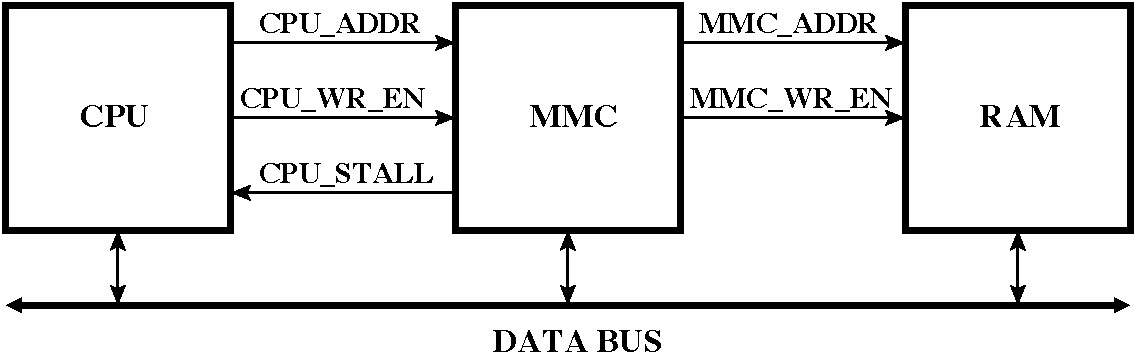
\includegraphics[height=0.5in, keepaspectratio=true]{figures/mmcramcpu.pdf} 
   \caption{Memory Map Controller (MMC)}
   \label{fig:mmcramcpu}
\end{figure}
%

The operations performed by MMC are three-fold.
%
First, it stalls the processor execution and takes control of the address bus to memory.
%
This occurs in the second cycle of the clock waveform shown in Figure~\ref{fig:mmcop}.
%
In the same clock cycle it performs an address translation operation to determine the address of the permissions in the memory map.
%
Address translation is shown in Figure~\ref{fig:memtrans}.
%
Memory map permissions are also read in this cycle as the MMC unit has control over the address bus.
%
Second, the MMC compares the ownership information to the identity of the current executing domain.
%
Finally, if the check is successful, then the MMC issues a write enable signal to the data memory.


The subset of address space protected by the memory map is defined by the register pair \texttt{mem\_prot\_bottom} and \texttt{mem\_prot\_top}.
%
The first step during translation is to determine the offset of the write address into the protected address space.
%
This is done by subtracting the lower bound of protected memory address space from the issued write address. 
%
Assuming a block size of 8 bytes, the nine significant bits of the address offset represent the block number.
%
Permissions are packed into a byte.
%
If the encoded information is stored in four bits (assuming multi-domain protection), then each byte would contain information of two contiguous memory blocks.
%
Therefore the last bit of the block number represents the byte offset of the permission.
%
The remaining bits index into the Memory Map Table.
%
The base pointer of the Memory Map Table is stored in a special register called \texttt{mem\_map\_base}.
%
The address of the permissions byte is computed by adding the memory map index to the memory map base pointer.
%
%
\begin{figure}[t]
  \centering
    \mbox{
      \subfigure[Timing]{\label{fig:mmcop}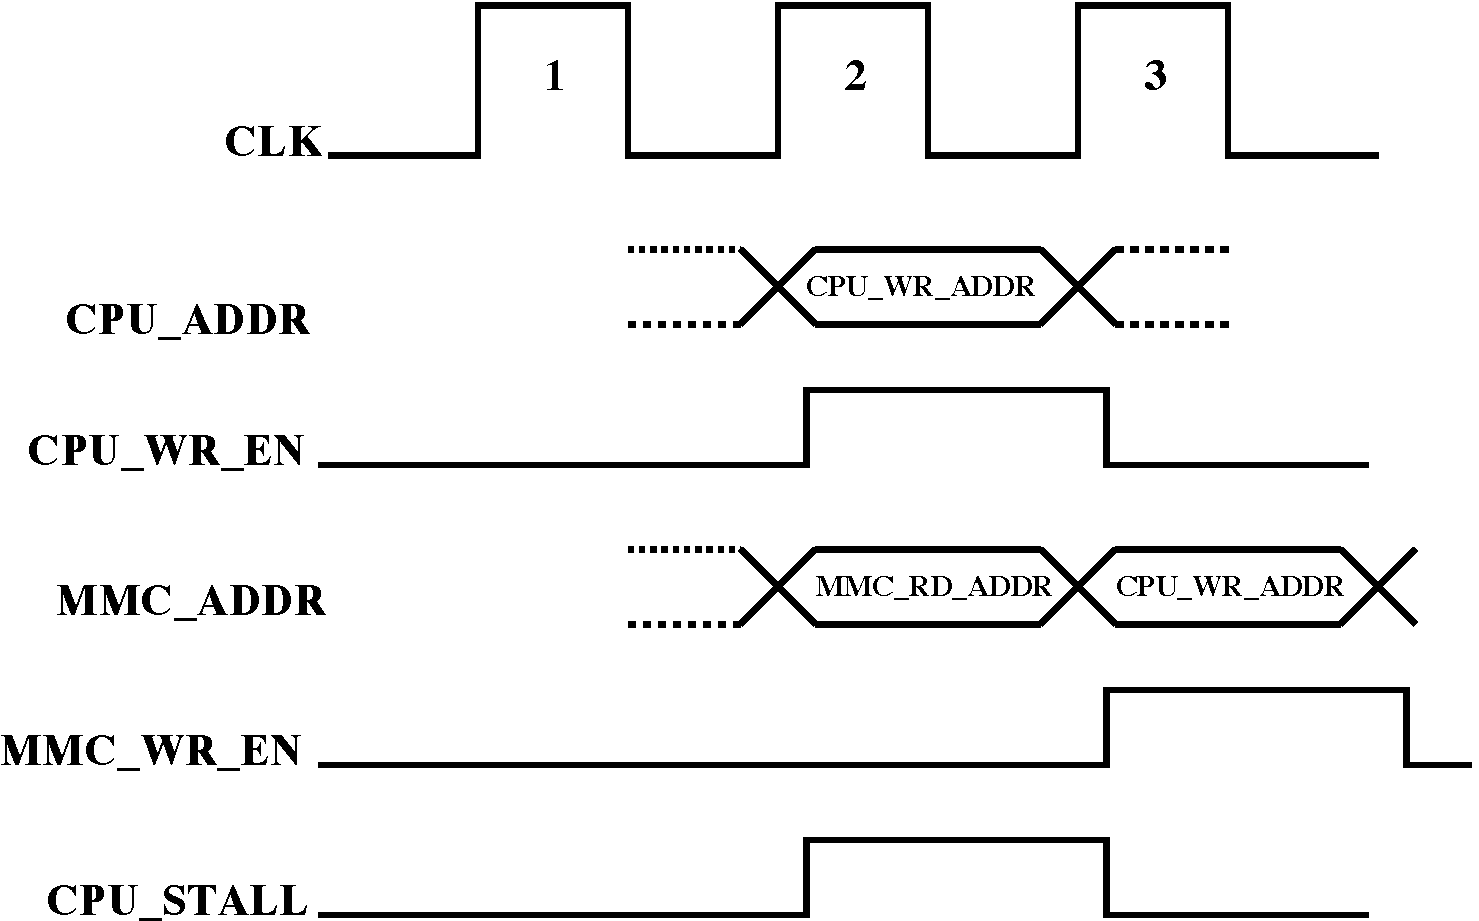
\includegraphics[height=1.2 in, keepaspectratio = true]{figures/mmcop.pdf}}\quad
      \subfigure[Addr Translate]{\label{fig:memtrans}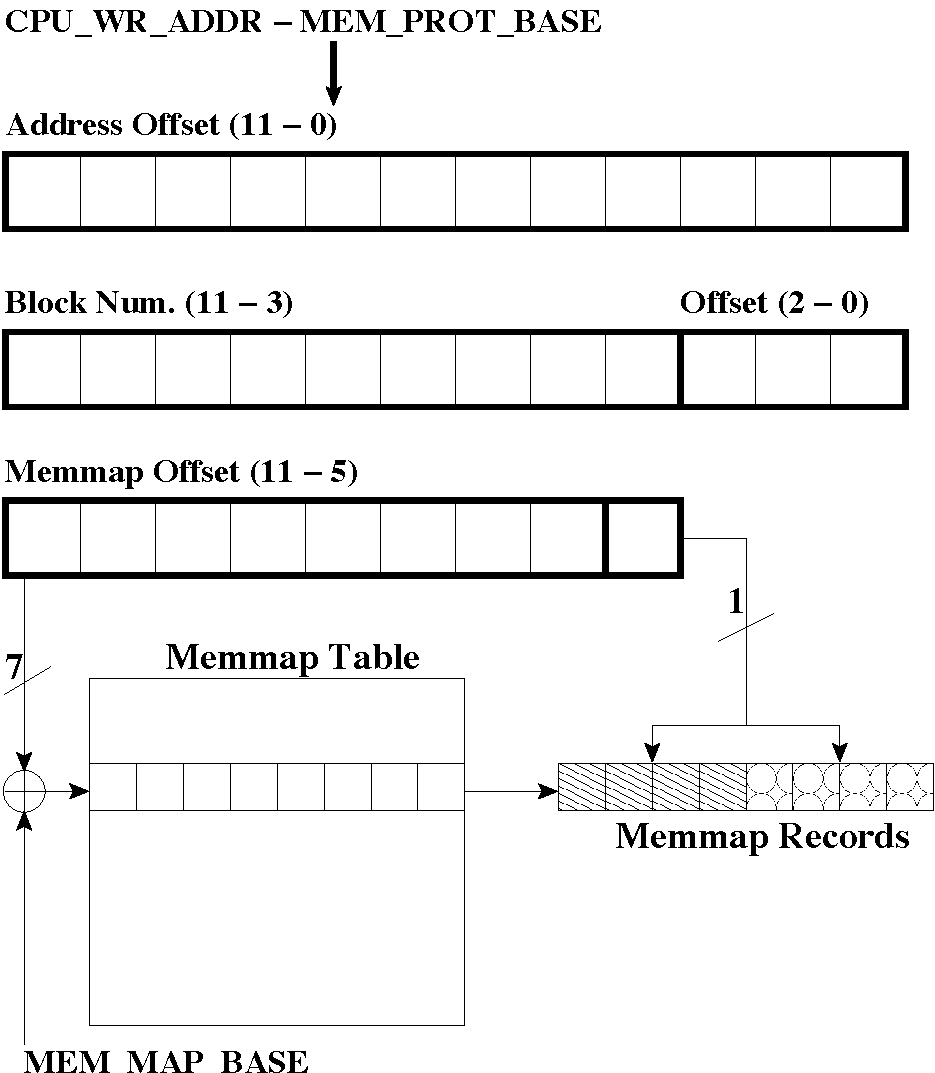
\includegraphics[height = 1.25in, keepaspectratio = true]{figures/memaddrtrans.pdf}}
    }
    \caption{MMC Operations}
    \label{fig:mmc}
\end{figure}

%
%
The Memory Map data structure is configurable through a set of programmable registers shown in Table~\ref{tab:mmap_config}.
%
The registers are accessible only by the run-time library loaded in the trusted domain.
%
The \texttt{mem\_map\_config} register is used to configure the block size and the number of protection domains available in the system.
%
\begin{table}[htdp]
\centering
\small{
\begin{tabular}{|l|l|}
	\hline
	Register & Function\\
	\hline
	\texttt{mem\_map\_base} & Memory map base pointer \\
	\texttt{mem\_prot\_bot} & Lower bound of protected address space\\
	\texttt{mem\_prot\_top} & Upper bound of protected address space\\
	\texttt{mem\_map\_config} & Configure block size and domains\\
	\hline
\end{tabular}}
\caption{Memory Map Configuration Registers}
\label{tab:mmap_config}
\end{table}
%
%========================================================================================================================================
% MEMORY MAP SOFTWARE LIBRARY
%========================================================================================================================================
\subsection{Memory Map Software Library}
\label{subsec:mmap_for_protection}
%
The software library manages all the memory available on the embedded processor.
%
First, it ensures that the memory map accurately reflects current ownership and layout.
%
In any real system, memory is constantly allocated, de-allocated or transferred from one module to another.
%
The Memory Map should be immediately updated when any of these events occur.
%
The library provides \texttt{malloc}, \texttt{free} and \texttt{change\_own} calls that automatically update the  Memory Map data structure. 
%
Second, it only permits the  block owner to free or change its ownership.
%
This condition is necessary as one module may (due to programming errors) free up memory that is being used by other module in the system.
%
Also it prevents a module from accidentally hijacking memory that is owned by other modules.
%
To enforce this condition, the software library reads the identity of the current active domain from the status register.
%
%We describe implementation details of tracking current active application in Section~\ref{sec:cfmgr}.
%
Third, the software library sets up the memory map to be located in a protected region of memory.
%
This prevents accidental corruption of the Memory Map data structure.
%
It is the responsibility of the software library to ensure that a memory map of sufficient size is allocated in the system.
%
Fourth, it initializes the MMC with the appropriate block size, number of protection domains and the range of protected address space.
%






%==============================================================================================
% CONTROL FLOW MANAGER
%==============================================================================================
\section{Control Flow Manager}
\label{sec:cross_domain_linking}
%
Programming errors can cause a module to corrupt its own state.
%
Protection domains created and enforced by the memory map manager cannot prevent such internal memory corruption.
%
Control flow within a system can be affected by internal memory corruption.
%
For example, function pointers (commonly used to implement callbacks) are stored in RAM.
%
Return addresses to function call-sites are stored in the stack.
%
Corruption of these values can cause the processor to execute arbitrary code belonging to the trusted domain.
%
%This violates one of the requirements of using memory map for protection; restricting memory map access to single trusted domain (Refer Section~\ref{subsec:mmap_for_protection}).
%
The Control Flow Manager ensures that control can never flow out of a domain except via calls to functions exported by other domains and via returns to calls from other domains.
%
Conversely, control flow can enter a domain only through an exported function or through the return site of a call that is made to a function exported by some other domain.
%
In addition, the identity of the current domain (that is executing) also needs to be tracked.
%
This information is required by the memory map checker to validate write accesses.
%
%We have implemented a Cross Domain Linking mechanism that is used to transfer control safely from caller to callee domain and vice versa.
%
%A corresponding Cross Domain Return mechanism restores control back to caller domain. 
%
Control flow integrity within a domain is preserved through the safe stack that stores return addresses.
%
%==============================================================================================
% CROSS DOMAIN LINKING
%==============================================================================================
\subsection{Cross Domain Linking}
%
A module loaded in a domain exports a set of functions that can be validly called by modules in other domains.
%
%Cross domain linking enables a module belonging to a domain to call functions in other domain.
%
%Modules in a domain are linked with modules in other domains at load-time.
%
A linker parses the set of functions exported by a domain and writes them to a \textit{jump table} in flash memory.
%
The jump table is similar in design to the processor interrupt vector table.
%
Each entry in the jump table is an instruction to jump to a valid exported function.
%
Each domain has its own jump table that contains all functions that it exports. 
%
Modules are not allowed to directly write to flash memory and therefore the jump table cannot be corrupted.
%
Modules that subscribe to functions exported by a particular domain are re-directed through the jump table of that domain.
%
This is illustrated in Figure~\ref{fig:cross_domain_call}.
%
The jump table mechanism is independent of the process used for dynamic linking i.e. exporting and subscribing to functions.
%
Linking could be done statically or dynamically on the embedded processor~\cite{dunkels06linking}.
%
\begin{figure}[htbp]
   \centering
   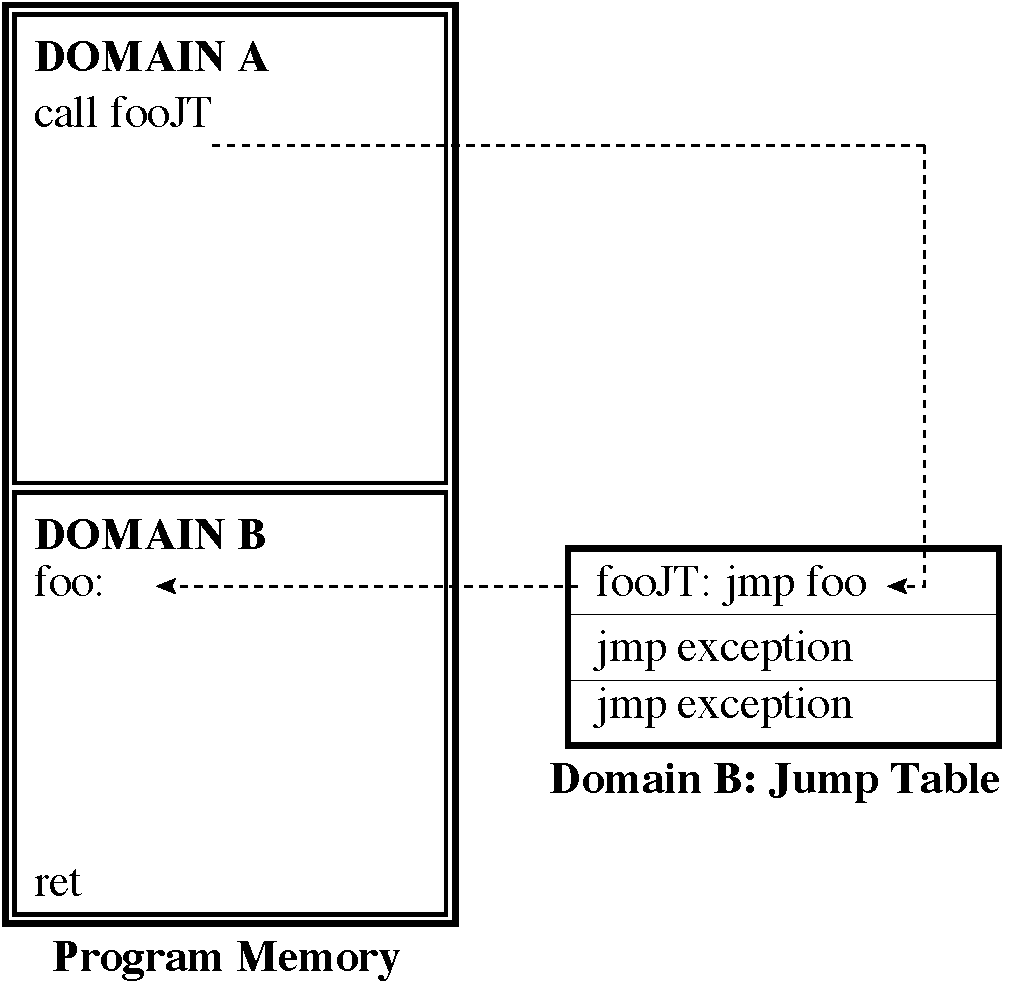
\includegraphics[height=1.75in, keepaspectratio=true]{figures/cross_domain_call.pdf} 
   \caption{Cross Domain Linking}
   \label{fig:cross_domain_call}
\end{figure}
%
%==============================================================================================
% DOMAIN TRACKING
%==============================================================================================
\subsection{Domain Tracking}
%
Domain tracking is performed in hardware by extending the implementation of \texttt{call} and \texttt{return} instructions.
%
Each domain is allocated one complete page of flash memory for storing its jump table.
%
In AVR architecture this imposes a limit of 128 functions that can be exported by every domain.
%
This limit can be easily extended by allocating more space to the jump table.
%
%The maximum number of exported functions by any SOS module is 12.
%
Empty entries in the jump table are filled with a jump instruction to an exception routine.
%
Jump table pages of all domains are co-located and stored at fixed location in flash memory.
%

This organization simplifies the algorithm for verifying the target address of a call.
%
A valid target address has to reside in the jump table.
%
This is checked by a simple compare operation to the base address of the jump table.
%
The check against the upper bound of jump table is deferred.
%
%and stack bound need to be stored in a stack.


The identity of the called domain is also easily determined.
%
Jump tables of all domains are organized linearly, starting from the domain 0 jump table located at the base address.
%
The identifier of the target domain can be easily determined by first computing the address offset from the base address of the jump table and dividing it by the size of the jump table.
%
If the target domain identifier exceeds the maximum number of domains in the system, then it indicates that the target address is greater than the upper bound of the jump table, and an exception is generated.
%
Finally, a call is made into the jump table that is redirected to the actual entry point in the target domain.
%

The current domain identifier needs to be pushed to a stack, because cross domain calls can be chained: domain A calls domain B which in turn calls domain C.
%
During cross domain return, the previous domain identifier is restored and the control is transferred back to the caller's domain.
%
The cross domain state machine handles the push and pop operations transparently to the application programs.
%
%All function calls made across domains pass through a \textit{jump table} setup in the program memory.
%
%Four operations are performed by the cross domain call stub.
%
%First, it verifies target address of the call.
%
%A valid target address should match the address of any exported function.
%
%Second, it determines the identity of callee domain and stores it.
%
%Third, it saves the return address of caller domain.
%
%Fourth, it sets up a stack bound.
%
%Stack bound is required for stack protection (Section~\ref{subsec:stackguard}).
%
%Cross domain call stub resides within the single trusted domain.
%
%Design of calling mechanism tries to optimize performance overhead of these operations.
%
%
%==============================================================================================
% STACK PROTECTION
%==============================================================================================
\subsection{Run-Time Stack Protection}
\label{subsec:stackguard}
%
Embedded micro-controllers have a single execution stack that is shared by the entire system.
%
In most architectures, the stack is initialized at the end of address space and grows down towards the start of address space.
%
The run-time stack is used for many purposes.
%
First, it is used to record the return addresses of function calls.
%
Second, it is used to set up data frames for storing local variables or function arguments that cannot be accommodated in registers.
%
Third, it is also used to store arguments for variadic functions.
%
Stack corruption is a serious problem.
%
Our protection model prevents corruption of the stack belonging to one domain by any module belonging to a different domain.
%
During a cross domain call  the processor copies the current stack pointer into a \texttt{stack\_bound} register. 
%
The previous stack bound is saved.
%a stack bound is setup before control is transferred from one domain to another.
%
The memory map checker compares the write address to the current stack bound and signals an exception if the address exceeds the stack bound.
%disallows writes to memory addresses greater than current stack bound.
%
%As shown in figure~\ref{fig:checker}, stack access checker is invoked if the write address points to stack.
%
%Stack access checker 
%
Therefore, modules belonging to a domain cannot corrupt the stack belonging to another domain.
%
%==============================================================================================
% SAFE STACK
%==============================================================================================
\subsection{Safe Stack}
%
A module can call any local function within its domain.
%
The return address of function calls are stored in stack and are protected from corruption from modules in other domains.
%
However, a programming error can cause a module to corrupt its own stack.
%
This cannot be prevented by protection domains.
%
Therefore, we store all return addresses in a separate stack that resides in a different protection domain.
%
We call this a safe stack.
%
%Entry (and exit point) of every local function in a domain is re-written to invoke a stub routine that pushes (and pops) return addresses into the Safe Stack.
%
%Safe Stack pointer is maintained as a global variable that is read (and written) before (and after) a sequence of push/pop operations. 
%
%Safe Stack is used to overwrite return address values in run-time stack.
%
%We do not modify run-time stack in any manner as it would corrupt data frames setup by functions for storing local data and function arguments.
%
A safe stack can be setup only by the software in the trusted domain by writing to the \texttt{safe\_stack\_ptr}.
%
The safe stack can be setup anywhere in data memory as long as it is protected from accidental writes and overflow.
%
We usually setup Safe Stack at the end of all global data in the system and make it grow upwards.
%
Run-Time stack and Safe Stack approach one another.
%
%Binary rewriter introduces the stubs to push and pop into Safe Stack.
%
%Therefore, all return addresses are checked.
%
%Domains occupy contiguous portions in program memory. 
%
%When the domain is loaded into a system, the Control flow manager records its start and end addresses.
%
%Return addresses are checked to ensure that they lie within bounds of the current domain; else an exception is raised.
%
%Similarly, all computed call addresses are also subject to an identical bounds check.
%
%Calls to static addresses are verified at load time.
%
%All checks are introduced through a binary rewriter.














%=========================================================================
% EVALUATION
%=========================================================================
\section{Evaluation}
\label{sec:eval}
In this section, we will analyze the protection benefits and overheads introduced by our methodology.
%
We have implemented the hardware components of our design by making extensions to the AVR instruction set architecture.
%
The VHDL model of the extended processor is synthesizable.
%
We have instantiated the processor on Xilinx Vertex 2 Pro XC2VP30 FPGA.
%
Our performance overheads are measured using Modelsim 6.0 simulator.
%
The software library and applications were compiled using \texttt{avr-gcc} cross compiler.
%
%\subsection{Micro-Benchmarks}
%
\subsection{Performance Overhead}
%
We first present micro-benchmarks that measure CPU overhead introduced by the protection mechanism.
%
Table~\ref{tab:microbmperf} contains the overhead of run-time checks present in our mechanism.
%
We compare our overhead with a completely software based approach to memory protection through binary rewrites proposed in~\cite{ram06emnets} for the AVR architecture.
%
The software based approach also introduces identical run-time checks except that they are implemented in assembly language without any modifications to the processor architecture.
%
The results clearly indicate the superior performance of run-time checkers implemented in hardware.
%
\begin{table}[htdp]
\centering
\small{
\begin{tabular}{|l|c|c|}
	\hline
	Function Name & AVR Extension & AVR Binary Rewrite\\
	\hline
	Memmap Checker & 1 & 65\\
	Cross Domain Call & 5 & 65\\
	Cross Domain Ret & 5 & 28\\
	Save Ret Addr & 0 & 38\\
	Restore Ret Addr & 0 & 38\\
	\hline
\end{tabular}}
\caption{Overhead (CPU cycles) of Memory Protection Routines}
\label{tab:microbmperf}
\end{table}
%

The high overhead of software based memory map checker is mainly due to complex bit shift operations that are required to translate write addresses to memory map lookup.
%
Cross domain call and return have an overhead of five clock cycles when implemented in hardware.
%
The overhead occurs because the current domain identity, stack bound and return address have to be pushed to the safe stack before they can be updated with new values.
%
The total information that needs to be pushed to the stack is five bytes and only one byte can be written every clock cycle.
%
Similarly on the cross domain return, the five clock cycles are expended in restoring the values read from the safe stack.
%
Saving and restoring return addresses to the safe stack does not introduce any added overhead.
%
This is because the hardware unit for safe stack simply takes over the address bus when the processor is pushing the return address to the run-time stack.
%
By stealing the address bus from the processor, the hardware unit is able to simply redirect the store of the return addresses to the safe stack.

Next we evaluate the software library.
%
Performance overhead is also introduced by updates to memory map during allocation, free and transfer of memory within the system.
%
Table~\ref{tab:malloc_comparison} compares the overhead of memory allocation routines in the presence and absence of the protection mechanism.
%
Relatively higher overhead of \texttt{change\_own} and \texttt{free} calls is due additional checks that are introduced to prevent illegal ownership transfer or freeing of memory blocks by non-owners.
%
\begin{table}[htdp]
\centering
\small{
\begin{tabular}{|l|c|c|}
	\hline
	Function Name & Normal & Protected \\
	\hline
	malloc  & 343 & 610\\
	free & 138 & 425\\
	change\_own & 55 & 365 \\
	\hline
\end{tabular}}
\caption{Overhead (CPU cycles) of memory allocation routines}
\label{tab:malloc_comparison}
\end{table}
%

\subsection{Resource Utilization}
%
Resource utilization can be partitioned into sections.
%
The resource utilization of the software library and the overhead of hardware checkers.
%

%
%Code memory usage increases by about 15\% in protected kernel relative to unprotected kernel.
%
%Increase is mainly due to memory map API and jump table used by cross domain call mechanism.
%
%There is no significant change in program memory usage going from two protection domains to multiple protection domains.
%
%Data memory usage increases by 5\% and 9.5\% in two-domain and multi-domain systems respectively, relative to unprotected kernel.
%
%This is the maximum possible overhead as the memory map stores layout and ownership information of entire address space.
%
Code and data memory usage of the software library is shown in Table~\ref{tab:swlibsize}.
%
Maximum memory map size is 256 bytes for multi-domain protection.
%
This represents an overhead of 6.25\%.
%
However, by modifying data layout, portion of address space that requires memory map for protection can be reduced.
%
For example, memory map can be configured only to protect the heap and safe-stack.
%
By abutting these two data-structures, size of memory map required can be reduced to 140 bytes for multi-domain protection.
%
For two domain protection, the overhead can be reduced to only 70 bytes (1.7\%).
%
The total code memory usage of the software library is only 3674 bytes (2.8\%).
%
\begin{table}[htdp]
\centering
\small{
\begin{tabular}{|l|c|c|}
	\hline
	SW Component & FLASH (B) & RAM (B)\\
	\hline
	Dynamic Memory & 1204 & 2054\\
	Memory Map & 422 & 256 \\
	Jump Table & 2048 & 0 \\
	\hline
\end{tabular}}
\caption{FLASH and RAM overhead of software library}
\label{tab:swlibsize}
\end{table}
%

The hardware overhead of our mechanism is shown in Table~\ref{tab:hwsize}.
%
These results were computed by synthesizing our processor on Xilinx ISE 8.2i.
%
Most of the additions to the core area are in the memory map decoder that maintains a barrel shifter to support arbitrary bit-shifts in a single clock cycles.
%
We can eliminate this overhead if the processor is synthesized for a fixed block size and number of protection domains.
%
The overall increase in the core area is about 32\%.
%
This represents a modest increase in the overall area of the chip as the core occupies only a small fraction of the overall area.
%
Bulk of the chip area is occupied by SRAM and FLASH memories.
%
\begin{table}[htdp]
\centering
\small{
\begin{tabular}{|l|c|c|}
	\hline
	HW Component & Ext. Gate Count & Orig. Gate Count\\
	\hline
	AVR Core & 22498 & 16419\\
	Fetch Decoder & 6783 & 6685\\
	MMC & 2284 & N/A \\
	Safe Stack & 1749 & N/A \\
	Domain Tracker & 541 & N/A \\
	\hline
\end{tabular}}
\caption{Gate count overhead of hardware extensions}
\label{tab:hwsize}
\end{table}
%







%=======================================================================
% RELATED WORK
%=======================================================================
\section{Related Work}
\label{sec:related}
%
Page-based virtual memory systems have become the dominant form of
memory management in the modern general-purpose computer systems.
%
While the process model of the virtual memory systems deliver protection for embedded applications, they also increase overhead in memory consumption and processor performance.
%
The memory consumption increases due to the need to store address translation tables.
%
The processor performance is impacted because the context switch has a high overhead; page tables have to be setup for the new context.
%
To improve performance of virtual memory, architectural features such as Translation Lookaside Buffers (TLBs) and virtual-mapped caches are used that further increase the area, cost and complexity of the chip.
%
For example, the addition of MMU and cache in an ARM7TDMI core~\cite{arm7tdmi} increases its area ten fold and its power consumption two fold. 
%
Therefore, current MMU designs will never be used in the low end price sensitive microcontrollers.

%
Memory protection units (MPU) provide hardware assisted protection in  embedded processors such as ARM
940T~\cite{arm940tds} and Infineon TC1775~\cite{inftc1775ds}.
%
MPU can statically partitions memory and set individual protection attributes for each partition.
%
The partitions are contiguous segments within the address space defined by a pair of base and bounds registers.
%
The protection model of MPU is not suited for the complex embedded
software (such as operating systems) running on low-end microcontrollers.
%
MPU defines only two protection domains viz. User-mode and Supervisor
mode.
%
This is sufficient for protecting the kernel from the applications but
not the applications from one another.
%
The static partitioning of address space into contiguous regions is
infeasible for the low-end microcontrollers with very limited memory
footprint.
%
Further, the number of partitions is also limited.
%
However, MPU has a lower memory footprint than UMPU because the
partitioning information can be stored in registers instead of
maintaining a memory map.
%
MPU introduces no performance overhead while UMPU incurs a single
clock cycle penalty for memory map accesses.
%


%
Mondrian Memory Protection (MMP)~\cite{witchel-asplos02-mondrian} inspects memory accesses at the instruction level from within the processor pipeline to provide word-level protection.
%
It uses fairly complex and expensive hardware extensions to reduce overhead of monitoring all accesses.
%
SafeMem~\cite{qin-hpca05-safemem} exploits existing ECC memory protection to guard memory regions and detect any illegal accesses through ECC violations.
%
However, these techniques significant resources to be performed on tiny embedded processors.

%
Hardware support for memory safe execution of embedded software was recently proposed in~\cite{divya06ccured}.
%
This technique uses CCured~\cite{ccured02necula}, a tool that generates type safe C programs through pointer inference techniques.
%
Extensions to the instruction set architecture speed up the run-time bounds checking operations performed by CCured.
%
Our techniques apply directly to machine instructions and are therefore agnostic to programming languages.
%
Also, our hardware extensions do not modify the processor instruction set architecture.
%
Hence, we can continue to use existing compilers.
%
Custom modifications to compilers can become the source of new bugs.
%

Many software based approaches for memory protection have been proposed.
%
Type-safe languages such as Virgil~\cite{titzer06virgil} can flag illegal accesses at compile or run-time.
%
They provide fine-grained memory protection of individual objects.
%
Type-safe languages do not interface with code written in non type-safe languages.
%
However, most of the software developed for embedded systems is written in unsafe languages such as C (or even assembly for low-level drivers). 
%
Popular programming language NesC~\cite{gay03nesc}, contains minimal extensions to C (such as the \texttt{atomic} keyword) to prevent race-conditions that can cause memory corruption.
%
ASVM~\cite{asvm05nsdi} can also be used for providing memory protection. 
%
Software-based fault isolation for embedded processors has been proposed in ~\cite{ram07harbor}.
%
All the software based approaches have a significantly higher overhead than custom hardware extensions.

%===========================================================================
% CONCLUSION
%===========================================================================
\section{Conclusion}
\label{sec:conclude}
%
In this paper, we have proposed a hardware software co-design approach for providing memory protection in tiny embedded processors.
%
Though we have implemented the protection technology for the AVR microcontroller, our general approach is applicable to other RISC architectures such as TI MSP or ARM.
%
Through a careful partitioning of the protection techniques, we have significantly improved performance by moving compute intensive operations into hardware.
%
Our hardware is very flexible, it can accommodate various configuration parameters.
%
The software library provides a standard programming interface.
%
Moreover, our approach does not modify the instruction set architecture of the processor; hence we do not need to modify the cross compiler.
%
These features ensure that our software library can be incorporated into existing projects with minimal modifications; a very practical benefit to the system developers.
%
We are still exploring the design space of possible protection architectures.
%
The resource utilization of our design can be further reduced by synthesizing hardware units that are pre-configured for a particular block size and number of protection domains.
%
An interesting area of future work is to explore software techniques such as virtual machines or type-safe languages  that can benefit from modest hardware extensions.
%
Software reliability is an emerging concern in the domain of tiny embedded processors.
%
Limited resources preclude the application of existing approaches used in desktop processors.
%
We believe that hardware software co-design techniques are a promising avenue to explore for creating robust software for tiny embedded processors. 


\footnotesize{
\bibliographystyle{abbrv}
\bibliography{ramthesis}
}

\end{document}
